%!TEX root = ../main.tex

\subsubsection{CAN protocol}\label{sub:CAN_protocol}\martin{Maybe should be given a different neame? Like HL protocol or naming convention?}
Due to the requirements of the on-kart network, it is decided to formulate a new protocol specifically for this project. The requirements are listed below.\\
\textbf{On-kart network requirements}:
\begin{itemize}
	\item Simple and easy to learn.
	\item Support for 16 nodes.
	\item Broadcast data.
	\item Variable data length - beyond 8 bytes per message
	\item Expandable.
	\item Commands: Start/stop broadcasting 
	\item Commands can be send to specific or all nodes
\end{itemize}

The basic CAN framework is retained for this protocol, and the protocol is really just a naming convention for the message ID. 

\begin{figure}[h!]
	\centering
	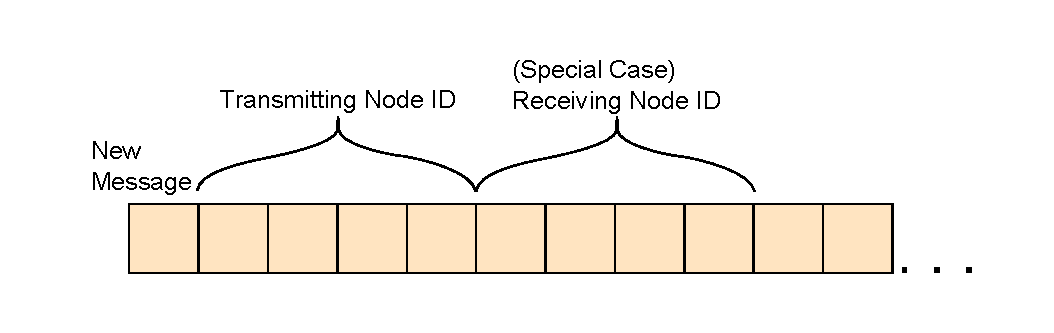
\includegraphics[width = 0.9\linewidth]{graphics/CAN_protocol_general_pdf}
	\caption{Naming convention for this high level protocol}
	\label{fig:CAN_protocol_general_pdf}
\end{figure}

The message ID is split in to three portions, as seen on figure~\ref{fig:CAN_protocol_general_pdf}.
The first bit is set to 1 if this is a new message.
If however the node needs to send more than 8 bytes in one package, this bit can be set to 0, thus blocking other nodes with higher priority.
The subsequent four bits indicate the transmitting node ID, which will allow up to 16 nodes. 
The last 6 bits of the message ID would determine the message type.
This message type then determines 
This leaves 64 different message types for each node -- it is then the developers to utilize these the best. 
If more message types are needed, the CAN protocol supports extended identifier, which adds 18 bits of identifiers.
This however also increases the overhead, and puts unnecessary load on the bus
Each node will have a list of message IDs (10 bits), that it knows how to handle.
If a message is not on that list, the node will ignore it.\\

There are basically two types of nodes: The Wifi node acting as a commander, and all other nodes.
Generally nodes can either produce data, and/or receive commands.
The Wifi node neither produces any kind of data nor receives commands, but it does receive data, and send out commands.
Therefore, there is a special case, for when the Wifi node is sending.
In this case, the subsequent four bits determines the recipient, leaving two bits for command type. 
For now, command types are only "Start broadcasting" and "Stop broadcasting", but could be extended to for instance "Set parameter" or "Set value", where the data field will indicate which parameter, and what is's set to.
If the recipient message ID is the WiFi node ID, then the command applies to all nodes.\\

The four node IDs are:
\begin{table}[h!]
	\begin{tabular}{{l} {l}}
		Wifi node: & 0b0001 \\
		IMU node: & 0b0011 \\
		Sevcon node: & 0b0111 \\
		GPS node: & 0b1110
	\end{tabular}
\end{table}
The reason for this naming is, that the Wifi node acts as a commander for the, and it's commands need higher priority.
The IMU produces short data packages at a high rate, and the GPS node produces longer data packages at a lower rate. 
Therefore it is of less concern if the GPS message is delayed due to obstruction from other nodes. 

\catalin{Based on Node ids and messages ids, is this useful or not?}
\subsubsection{Publisher-Subscriber Architecture}
\catalin{Should I explain more about the architecture? Or is it the readers responsibility to read about it?}
A mechanism was also necessary to control the receivers and transmitters of messages.
One of the functionalities of the network was to provide the ability for various nodes to be able to send specific messages to other nodes.
Such a mechanism could easily be implemented using the Publisher-Subscriber architecture which would also make the network data-driven.
Using this method, the communication among the various nodes could be easily configured just by adding messages ids to an array variable containing the node's subscriptions.
The use of this architecture was incorporated in the protocol functionality, along with a set of functions in the source code.
\paragraph{Implementation in code}
This was achieved by implementing a set of functions and an array variable of subscriptions for each node.
The important mechanisms that needed to be provided by the source code were the creation of the message id, the decoding of it as well as getting the various portions such as the node id and the message type.
The figure \ref{fig:SeqDiagram_SendFrame} shows the procedure of sending a frame containing data, which makes use of the protocol function createMsgID().

\begin{figure}[h!]
	\centering
	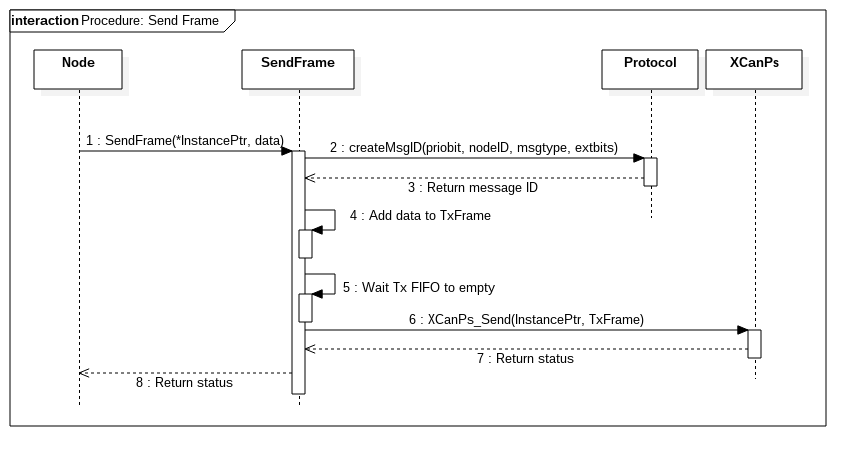
\includegraphics[width = 1.2\linewidth]{graphics/seqDiagram_SendFrame.png}
	\caption{The sequence diagram of the process of sending a frame.}
	\label{fig:SeqDiagram_SendFrame}
\end{figure}
\catalin{Receive Frame SeqDiag UNFINISHED}
\begin{figure}[h!]
	\centering
	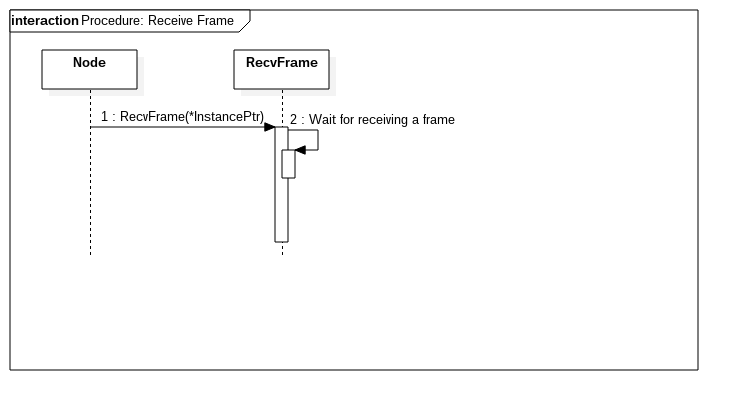
\includegraphics[width = 1.2\linewidth]{graphics/seqDiagram_RecvFrame.png}
	\caption{The sequence diagram of the process of receiving a frame.}
	\label{fig:SeqDiagram_RecvFrame}
\end{figure}
\catalin{Modify the two seq diagrams after a final discussion on the CAN protocol}
\catalin{Refer to the code in the appendix or place the function here.}